The communication is in the center of the hole system. Isolated, an agent is useless and it needs to share information in order to become powerful. Agents communicate together with a defined code. This section will explain the different type of messages and their role in the all system. The figure \ref{fig:communication_flows} summarizes the different messages and how agents exchange them.\\

\begin{figure}[h!]
    \centering
    \includegraphics[page=3,clip,width = 8cm]{systeme_multi_agent/conceptualization/multi_agent_schematic.pdf}
    \caption{Communication flows between agent}
    \label{fig:communication_flows}
\end{figure}

\notreVocabulaire{Heartbeats} messages are the simplest one but rather essential. In the schematic they are shown by the yellow arrows. In fact there is no exchange of information about targets or agents however it allows modularity in the system. At the start each agent considers all the other as inactive but as soon as it receives \notreVocabulaire{Heartbeats}, they will start to operate together. Now let's imagine an agent stops suddenly working well and therefore stop sending messages, then it will be set back as inactive by the others. The problem is though detected and the remaining agents can try to compensate this loss. Nevertheless as soon as it recovers and sends \notreVocabulaire{Heatbeats} again, then the others will set it back to active and the situation is restored to the point before the problem happends.\\

\notreVocabulaire{Related targets information} are use in every cases. The main goal is to share data either to synchronise the believes or to bring redundancy to be able to filter the data.\\

\notreVocabulaire{Related agents information} are used only when sensors can move in space. It creates a need to update the believes about other agent configuration because it can varies with respect to time. 

